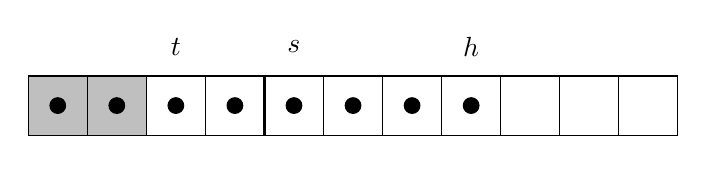
\begin{tikzpicture}[scale=0.75]
\draw[rectangle, color=black, fill=lightgray]  (-1,0) rectangle (0,1);
\draw[rectangle, color=black, fill=lightgray]  (0,0) rectangle (1,1);
\draw[rectangle, draw]  (1,0) rectangle (2,1) node (v1) {};
\draw[rectangle, draw]  (2,0) node (v2) {} rectangle (3,1);
\draw[rectangle, draw]  (3,0) rectangle (4,1);
\draw[rectangle, draw]  (4,0) rectangle (5,1);
\draw[rectangle, draw]  (5,0) rectangle (6,1);
\draw[rectangle, draw]  (6,0) rectangle (7,1);
\draw[rectangle, draw]  (7,0) rectangle (8,1);
\draw[rectangle, draw]  (8,0) rectangle (9,1);
\draw[rectangle, draw]  (9,0) rectangle (10,1);

\draw[rectangle, very thick, draw]  (3,-0) rectangle (3,1);

\node[circle, fill, draw, inner sep=2pt] at (-0.5,0.5) {};
\node[circle, fill, draw, inner sep=2pt] at (0.5,0.5) {};
\node[circle, fill, draw, inner sep=2pt] at (1.5,0.5) {};
\node[circle, fill, draw, inner sep=2pt] at (2.5,0.5) {};
\node[circle, fill, draw, inner sep=2pt] at (3.5,0.5) {};
\node[circle, fill, draw, inner sep=2pt] at (4.5,0.5) {};
\node[circle, fill, draw, inner sep=2pt] at (5.5,0.5) {};
\node[circle, fill, draw, inner sep=2pt] at (6.5,0.5) {};

\node at (1.5,1.5) {$t$};
\node at (6.5,1.5) {$h$};
\node at (3.5,1.5) {$s$};

\end{tikzpicture}